\subsection{The O-Crab Design} \label{subsec:solution}

The general assembly of the O-Crab locomotion and chassis is shown in Figure \ref{fig:general}. The robot recharges using Maxeon SunPower Solar cells on the top of the chassis \cite{sunpower_solar_2018}. 

Due to the nature of the robot's application, the chassis is constructed of acrylic as it is UV stable, resistance to cold weather and salt, and relatively strong \cite{marla_acme_best_2019} \cite{curbell_plastics_uv_2019}. Safety orange was selected for high visibility. It was designed to be fully sealed from the elements (sand, moisture, salt, dust, etc). This was achieved by the use of molded silicone bellows at the leg joints, which are flexible enough to allow the repeating angular motion of the legs \cite{custom_rubber_corp_rubber_2019}. Another aspect of sealing is the use of a compressed gasket between the chassis and its lid \cite{protocase_custom_2019}. This feature is shown in Figure \ref{fig:gasket}, where the gasket is positioned inside a groove which protrudes upward, creating a further barrier for water and particles. To prevent vandalism, tamper resistant bolts were used for the lid of the robot, making it difficult to dismantle \cite{mcmaster-carr_tamper_2019}. Furthermore, any fasteners penetrating the chassis (other than those holding the lid due to the gasket) have a compressed o-Ring to prevent water and contaminant ingress through the hole \cite{fastenright_sealing_nodate}. 


\begin{figure}[H]
    \centering
    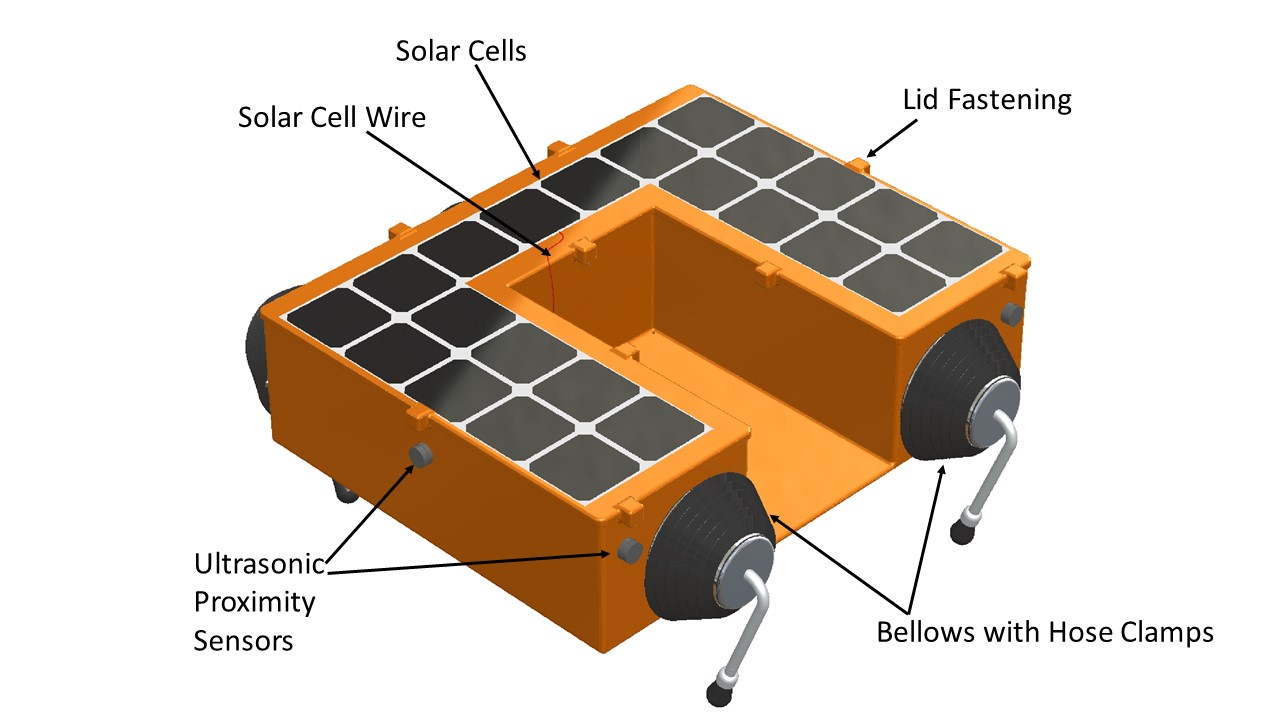
\includegraphics[width=\textwidth]{2_ProposedDesign/img/IsoViewA.jpg}
    \caption{O-Crab general assembly without litter system}
    \label{fig:general}
\end{figure}

\begin{figure}
    \centering
    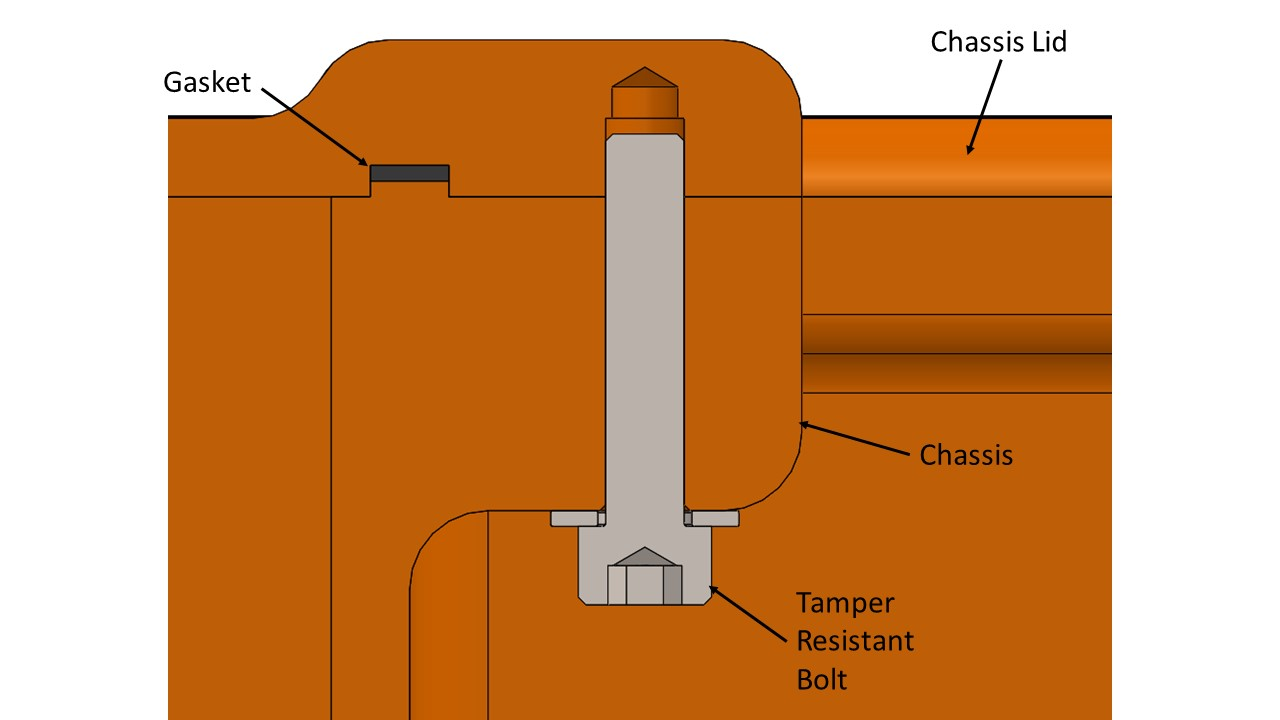
\includegraphics[width=\textwidth]{2_ProposedDesign/img/LidSectionA.jpg}
    \caption{Chassis gasket}
    \label{fig:gasket}
\end{figure}

\subsubsection{Electronics}

The robot is also equipped with sensor equipment, enabling independent operation and navigation of its environment. Ultrasonic proximity sensors are mounted through all four sides of the chassis to detect nearby objects. \cite{maxbotixs_mb7395_2017}. This will allow it to avoid obstacles and people \cite{corrigan_12_2019}. The motors each have a built in hall sensor for leg position and velocity control \cite{maxon_motor_maxon_2014}.


Other sensor equipment is found inside the chassis. 
A GPS/IMU unit from Inertial Sense allows for programming way-points, path-planning and retrieval assistance in case the robot becomes damaged or stolen \cite{inertial_sense_ins+rtk_2019}.
The IMU, or inertial measurement unit, detects orientation and acceleration of the chassis and will be used in the control system \cite{unmanned_systems_technology_selecting_2018}.

These elements are shown in Figure \ref{fig:chassis_topview} which shows a top view of the robot, with the chassis lid removed. Other elements shown in the top view are the controllers. An NVIDIA Jetson TX2 Module leverages its GPU to perform computer vision tasks and GPU based SLAM \cite{nvidia_jetson_2015} \cite{larabel_benchmarks_2017}. A Raspberry Pi 4 B is used for all other functions of the robot such as the overall control loop and communication \cite{raspberry_pi_raspberry_nodate} \cite{raspi.tv_how_2019}. oDrives power the leg and arm motors. Each one can control two motors simultaneously and allows for over 100A draw at 48V, well within operating conditions \cite{weigl_madcowswe/odrivehardware_2019}.

Also visible in Figure \ref{fig:chassis_topview} are the batteries and battery management system. The batteries stock energy from the solar cells for when the robot is operating, and are composed of Panasonic NRC18650B cells \cite{18650batterystore_panasonic_2019}. The battery management system ensures acceptable charge and discharge rates between cells \cite{voltaplex_6s16s_nodate}. As shown in the top view, the cells are split into two batteries, one on either side of the robot to distribute the weight more evenly.


\subsubsection{Leg Configuration and Movement}

Figure \ref{fig:chassis_topview} also shows the leg configuration (note that some of the timing belts were removed to show other leg details). Three legs are placed at the back and two at the front, with the litter and robot arm between them (see Section \ref{subsec:interconnectivity}).
The legs have two degrees of freedom, allowing them to extend in and out. A third degree of freedom for rotation of the leg around the vertical axis of the robot was not added to reduce complexity. The robot turns by moving legs on one side (right or left) faster than the other side. 
The two front legs are positioned as close to each other as possible. This makes the robot more stable, as shown in the stability triangle analysis of the Modelling Report. 

\begin{figure}
    \centering
    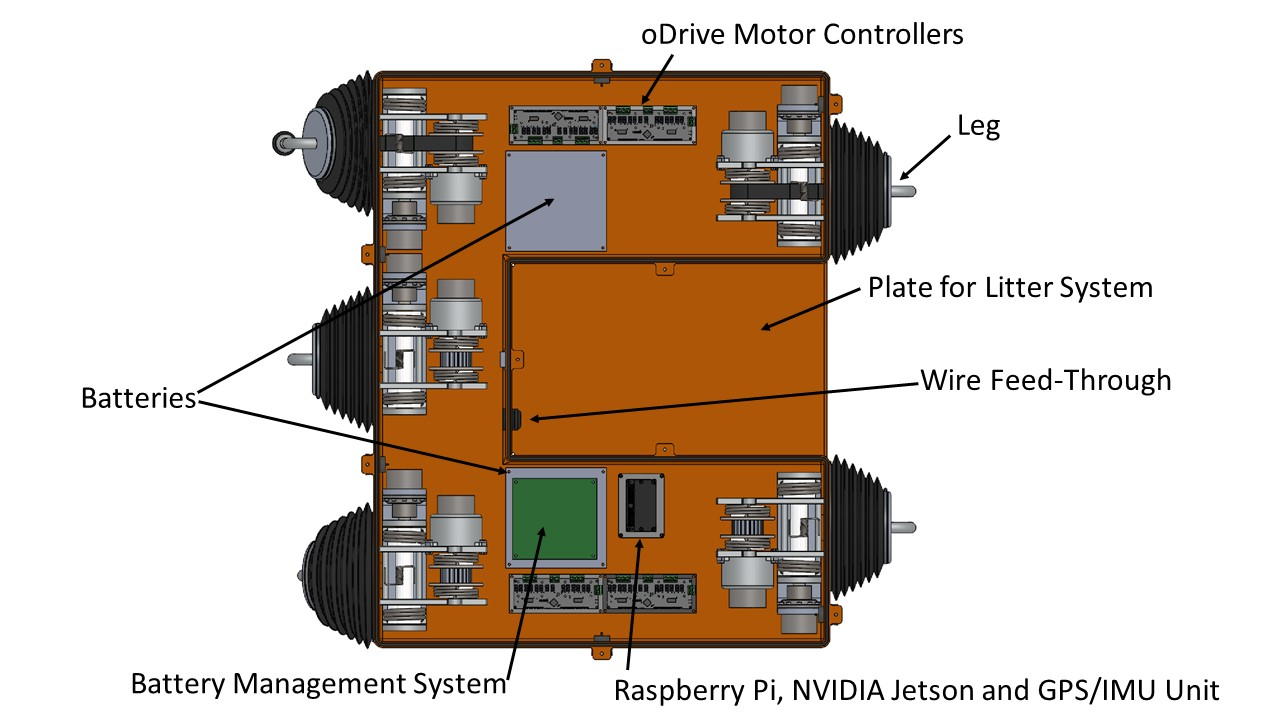
\includegraphics[width=\textwidth]{2_ProposedDesign/img/TopViewA.jpg}
    \caption{Top view of component layout inside the chassis}
    \label{fig:chassis_topview}
\end{figure}



\begin{comment}

***THIS PART OF THE REPORT HAS BEEN REMOVED***

Figure \ref{fig:chassis_sideview} shows a side view of the chassis with legs positioned at two different positions. The leg on the RIGHT is in the most extended position and the leg on the LEFT is in the least extended position of the walking gait. The joint angles are limited to $0^{\circ}$ to $28^{\circ}$ from horizontal for the thigh linkage and $-22.5^{\circ}$ to $22.5^{\circ}$ for the tibia linkage, relative to the thigh. This was selected in order to not over-extend the bellows. Only a subset of all possible leg positions is used while walking in order to conserve energy; this is explained in greater detail in Section \ref{app_sub:linkages}.
The linkages $r_1$, $r_2$ and $r_3$ change in length with parameterization inputs, but always keep the same ratios relative to each other as determined experimentally in Section 3.4 of the Analysis Report. The value of $r_1$ is the distance between the hip control shaft and the exterior knee shaft (see shafts referenced in Figure \ref{fig:leg_sideview}), $r_2$ is the upper part of the tibia before the bend and $r_3$ is the lower part of the tibia including the foot assembly. 

\begin{figure}
    \centering
    \includegraphics[width=\textwidth]{SideviewWithAnglesAndLinkNames}
    \caption{Side view of chassis and leg positions}
    \label{fig:chassis_sideview}
\end{figure}

\end{comment}



\subsubsection{Major Leg Components}

Figure \ref{fig:foot} shows a section view of the foot assembly. The semi-spherical elongated shape was chosen to ensure the foot would not dig in deep or get caught in mud or sand. A flexible silicone "sock" was chosen as the outer material to provide some damping to the legs. Its flexibility also allows it to be slipped on and secured in the ridge on the foot rod by use of its elasticity. Once installed, it is further secured by a cap which is screwed down onto the outer portion of the silicone. This cap would have been installed on the foot rod, which is manufactured with a threaded portion, prior to installing the silicone sock. The foot assembly is then press fit into the tibia tube. 

\begin{figure} [H]
    \centering
    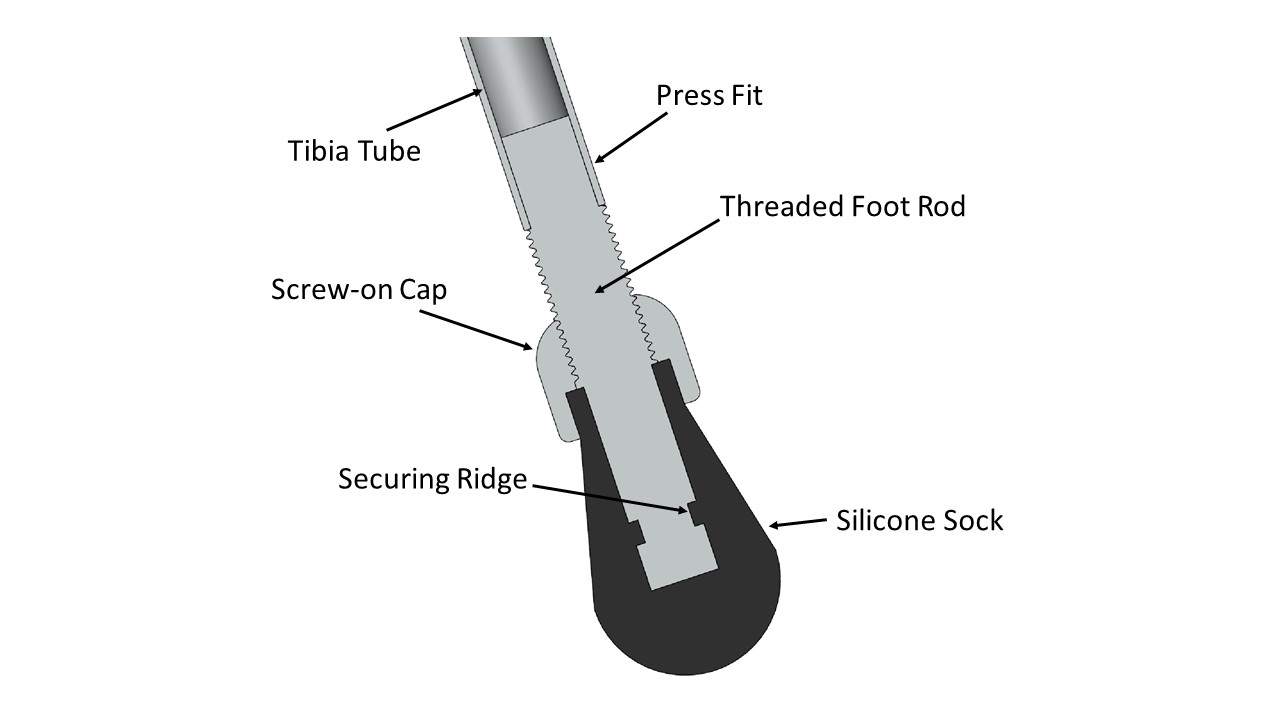
\includegraphics[width=\textwidth]{2_ProposedDesign/img/SectionFootA.jpg}
    \caption{Section view of foot assembly}
    \label{fig:foot}
\end{figure}

As shown in the leg section side view of Figure \ref{fig:leg_sideview}, the robot uses a belt and pulley system to rotate the knee, reducing the inertia of the leg and the required bellow size by keeping the Harmonic Drives and motors within the chassis. A steel reinforced HTD8 urethane timing belt was used for synchronisation and to prevent slipping \cite{gates_mectrol_urethane_2018}. To facilitate assembly of the belt and ensure that belt stretching with temperature and usage is compensated, a small torsion spring tensioner is added directly onto the belt shown in Figure \ref{fig:leg_topview}. As the movement of the leg is oscillatory instead of performing full rotations, this spring is positioned as to not interfere with the pulleys. 

The bellow is attached to the chassis using a hose clamp around a protruding circular flange on the chassis. The other end of the bellow is attached to the tibia holder, which simultaneously connects the bellow, the exterior knee pulley and the tibia tube. The tibia holder's large diameter is required for the bellow, as it needs to be larger than the hypotenuse of the shaft length and thigh plate height. It has two "arms" extending out which are bolted to both sides of the pulley, shown in Figure \ref{fig:leg_topview}. The tibia holder must be relatively thick as the tibia tube is press fit into it. Thus, some material was removed between the various features, as the outer portion holding the bellow does not take much force. The tibia tube was chosen as an aluminum circular tube to remain lightweight.

\begin{figure}
    \centering
    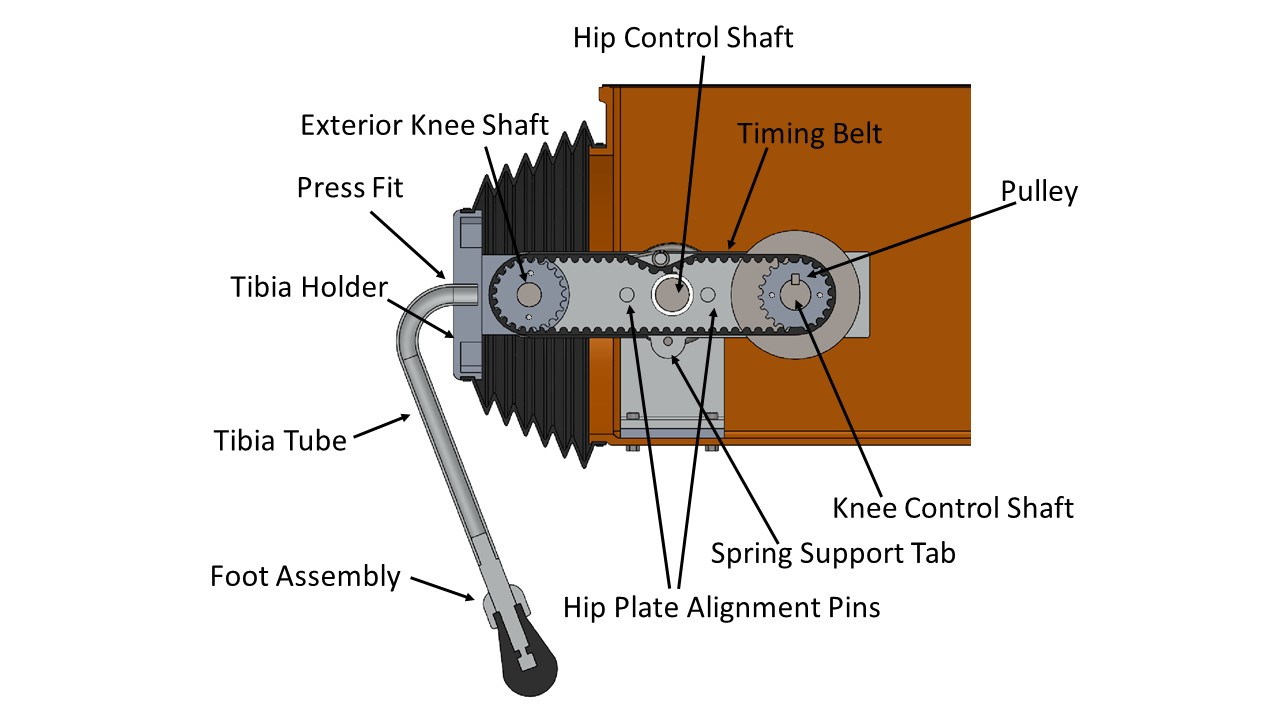
\includegraphics[width=\textwidth]{2_ProposedDesign/img/LegSectionWithBellowA.jpg}
    \caption{Side section view of leg showing belt assembly}
    \label{fig:leg_sideview}
\end{figure}

Figure \ref{fig:leg_topview} shows a top view of the thigh portion of the leg without the chassis or bellow. Contrary to the tibia hollow tube, it consists only of two two hip plates. This design was chosen as it takes less space than a circular tube for the same size of belt system. It also makes the leg easier to assemble and reduces the complexity of the leg. The plates are made relatively thick to support the exterior knee shaft, knee control shafts and to be able to fix them onto the hip shaft with keys.

Alignment pins for the hip plates are found on either side of the hip control shaft. They extend from one hip plate and are inserted into holes inside the other hip plate. They allow the holes for the shafts to be machined simultaneously in the correct final plate position, ensuring proper shaft alignment. Their second purpose is also to provide some additional structure to the hip plates, and to secure the plates together by using a bolt at the end of each pin.

Both the hip control shaft and knee control shaft are connected to a Harmonic Drive reducer and electric DC motor \cite{harmonic_drive_csd-2a_2019} \cite{maxon_motor_maxon_2014}. The motor and Harmonic Drive connected to the knee control shaft are mounted directly to the hip plate using the knee adaptor, with the Harmonic Drive hidden inside the adaptor. This entire assembly moves with the hip plates.

Torsion springs are positioned on the hip control shaft and knee control shaft. While the legs are not moving, the joint torques are brought below the Harmonic Drive non-backdriving torque, allowing them to passively hold up the robot. This solution provided significant power savings, as the robot generally moves only one leg at a time off the ground. The only drawback with this solution is that the moving leg will have to use more energy to fight the springs, however, this value is much less than constantly having all legs powered. Two identical but mirrored springs were used for each shaft, as this provided springs of smaller diameter, making the hip plates more compact and the shaft assemblies more symmetrical. 

\begin{figure} [H]
    \centering
    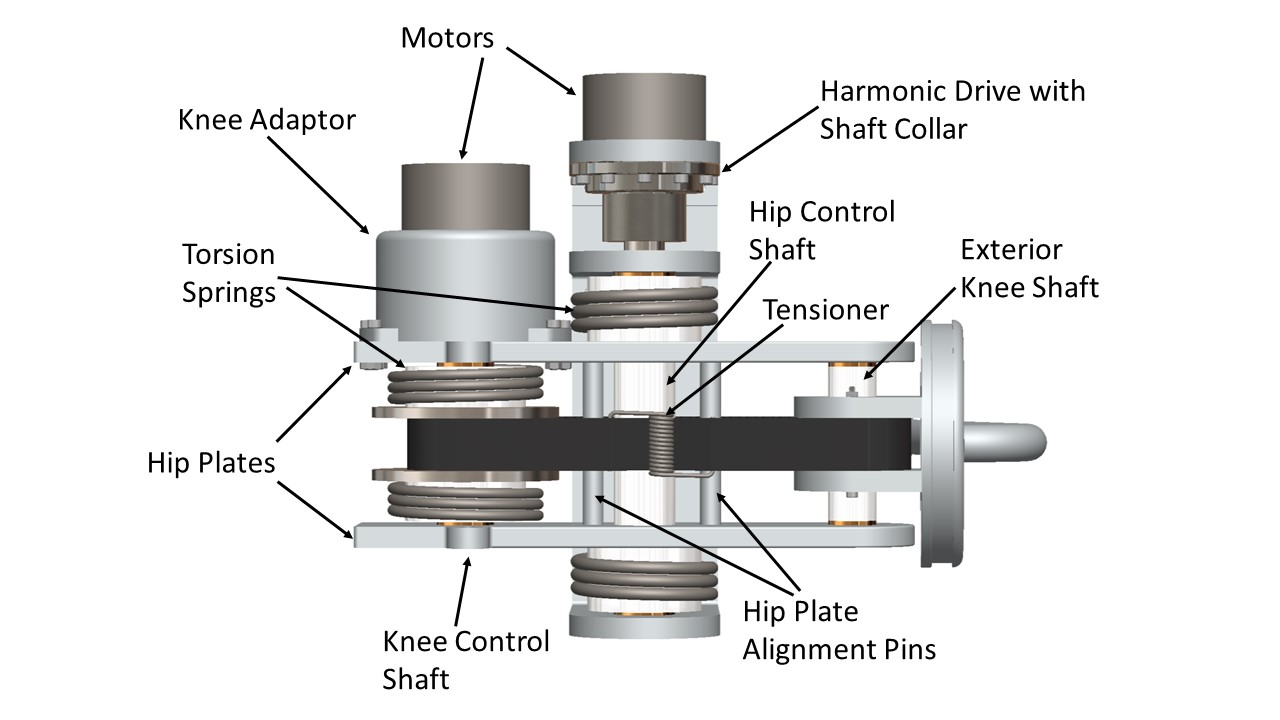
\includegraphics[width=\textwidth]{2_ProposedDesign/img/LegTopViewA.jpg}
    \caption{Top view of leg thigh without chassis or bellow}
    \label{fig:leg_topview}
\end{figure}


\subsubsection{Leg Shafts Assemblies}

Figure \ref{fig:shaft_knee} shows a section view of the exterior knee shaft and its components. Spacers are used to position the components axially. The pulley has no key as it is directly connected to the tibia holder using bolts. The exterior knee shaft is only structural and does not transfer any torque.
The shaft is supported by sintered bronze sleeve bearings with flanges \cite{qbc_bearings_flanged_2019}. The other shafts are also supported by sleeve bearings as shown in Figures \ref{fig:shaft_hip} and \ref{fig:shaft_kneehip}. These were selected over ball or needle bearings as the legs are often static, and radial forces on the shafts were quite high due to the belt tensions and forces from the legs. The flanges were added to prevent the shaft step and spacer from rubbing on the plates and to position the sleeve bearings in the plates. 

\begin{figure}[H]
    \centering
    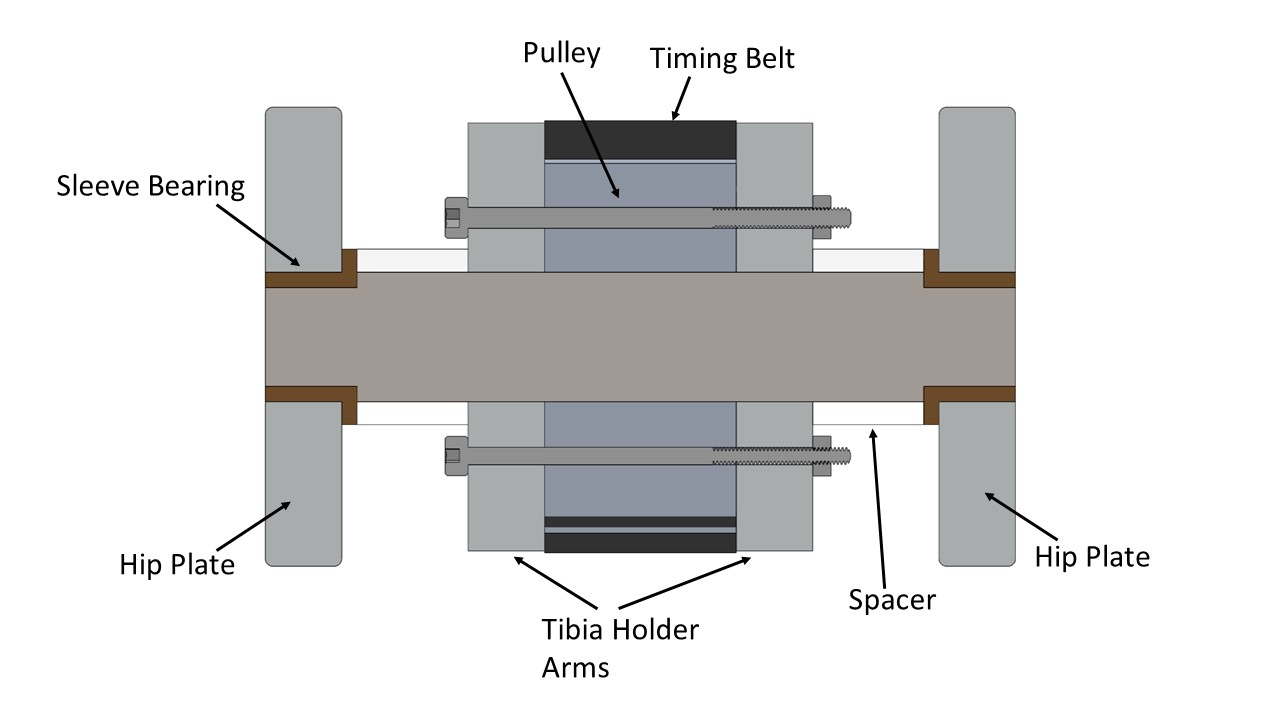
\includegraphics[width=\textwidth]{2_ProposedDesign/img/SectionKneeShaftA.jpg}
    \caption{Section view of exterior knee shaft}
    \label{fig:shaft_knee}
\end{figure}

Figure \ref{fig:shaft_hip} shows a section view of the hip control shaft, its components and the brackets and adaptor used to support it. The hip plates are held on the shaft by keys and are axially positioned by spacers. The spacers at the springs are larger to support the springs as they move. 

The shaft is supported by two L-brackets which are attached to a base plate, which is then attached to the chassis. One end of the springs connect to the hip plates and the other connects to its corresponding L-bracket. If the spring is larger than the hip plate height, a "tab" of additional material is added on the hip plate instead of increasing its total height, which would increase the size of other parts. This detail is shown in Figure \ref{fig:leg_sideview}.
To allow for the proper alignment of the hip control shaft, the L-brackets each have two alignment pins at their base which are positioned into holes on the base plate. This assembly is shown in Figure \ref{fig:hip_bracket}. To support the motor and Harmonic Drive, an adaptor piece was created, and extends down to the base plate. It has a similar shape to the L-brackets and uses alignment pins as well. The motor is mounted first onto the adaptor, then the Harmonic Drive.

The shaft collar used to connect the output of the Harmonic Drive to the hip control shaft is also of interest. As the stainless steel shafts are larger in diameter than typical steel shafts would have been, a regular flange collar did not work for the connection, as the Harmonic Drive flexspline bolt holes are quite close together. A flange-less and slightly thicker custom collar was thus created for the purpose of this application.

\begin{figure}
    \centering
    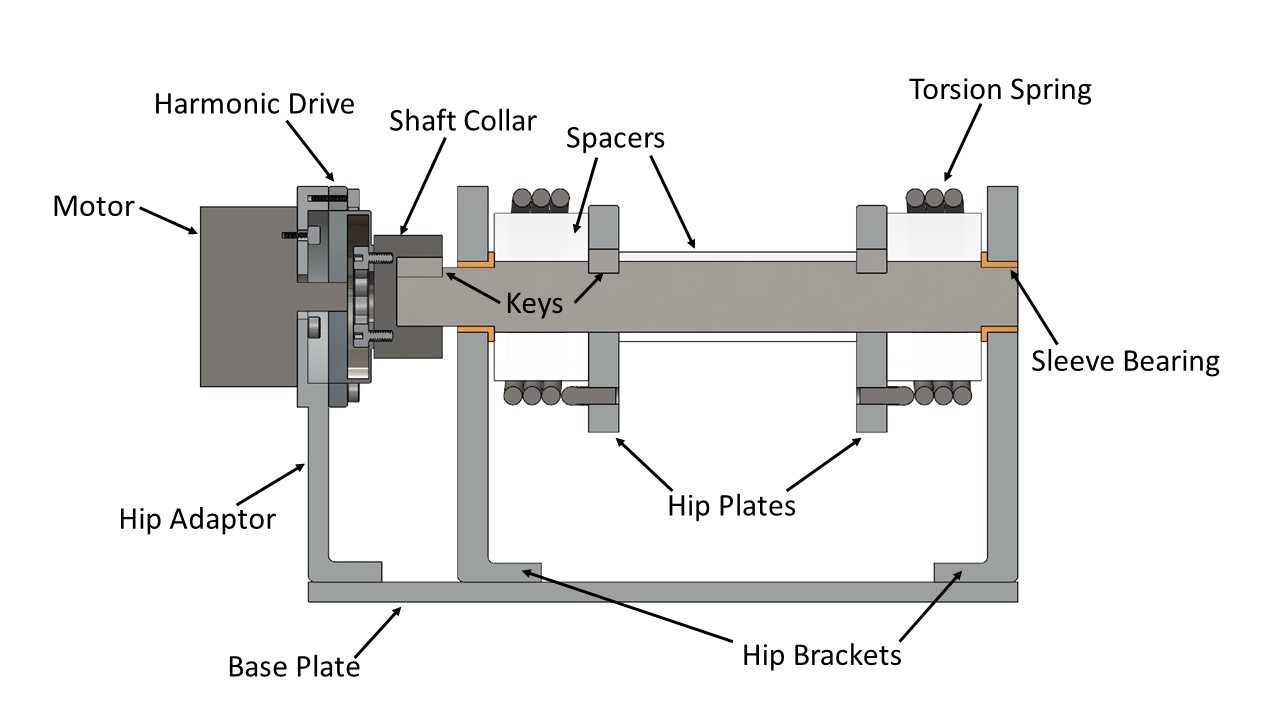
\includegraphics[width=\textwidth]{2_ProposedDesign/img/SectionHipShaftA.jpg}
    \caption{Section view of hip control shaft and its supporting brackets and adaptor}
    \label{fig:shaft_hip}
\end{figure}

\begin{figure}
    \centering
    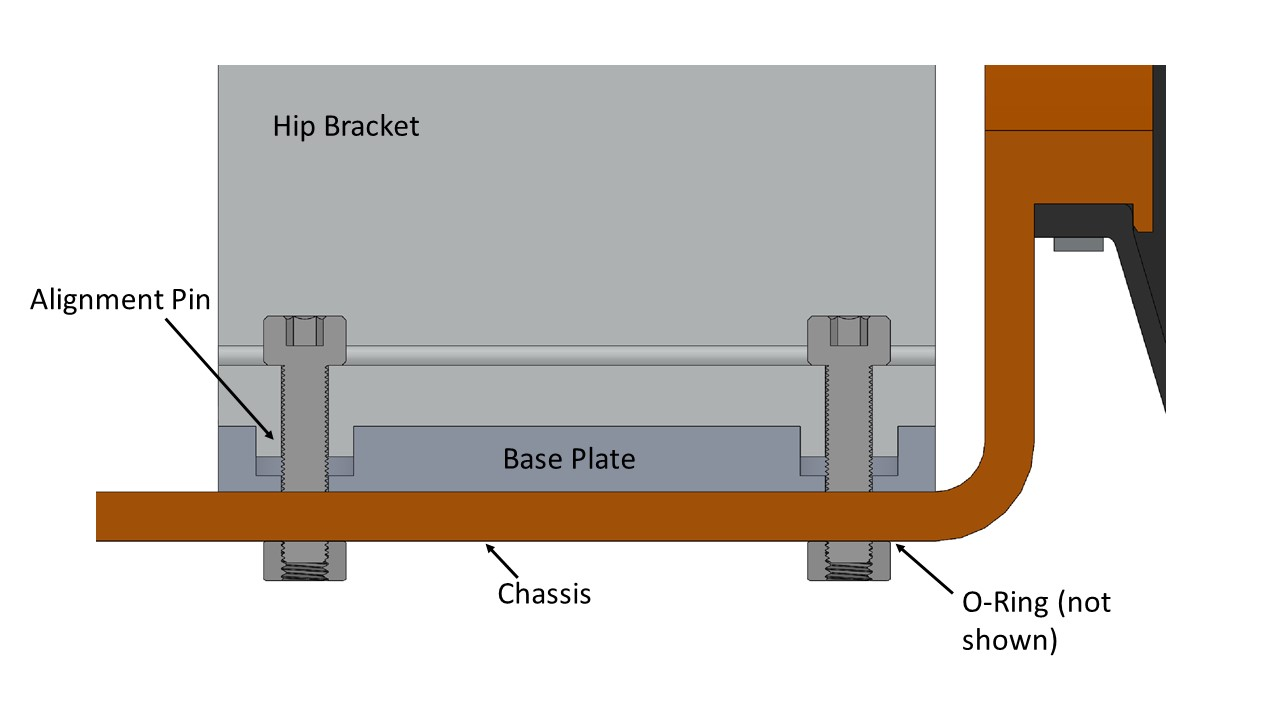
\includegraphics[width=\textwidth]{2_ProposedDesign/img/AlignmentPinsZoomedInA.jpg}
    \caption{Section view of hip bracket alignment pins and fastening to chassis}
    \label{fig:hip_bracket}
\end{figure}

Figure \ref{fig:shaft_kneehip} shows a section view of the knee control shaft, its components and the adaptor used to support its motor and Harmonic Drive. The knee adaptor uses a similar configuration to the adaptor at the hip control shaft, but attaches to the hip plate instead of the base plate and chassis. The pulley uses a keyway as this shaft transmits torque, unlike the exterior knee shaft. A pulley plate is attached on either side of the pulley (fasteners are not visible in this view as they were made to be offset from the keyway). The purpose of these parts is to provide a surface on which to attach the torsion springs. The other side of the springs is attached on the hip plates (with an added "tab" if required, as with the hip springs). Once again, a larger spacer is used to support the spring. Pins are used to fasten the pulley plates to the pulley instead of bolts to avoid interference. As with the hip control shaft, a custom shaft collar is used to attach the Harmonic Drive output to the shaft.

\begin{figure}
    \centering
    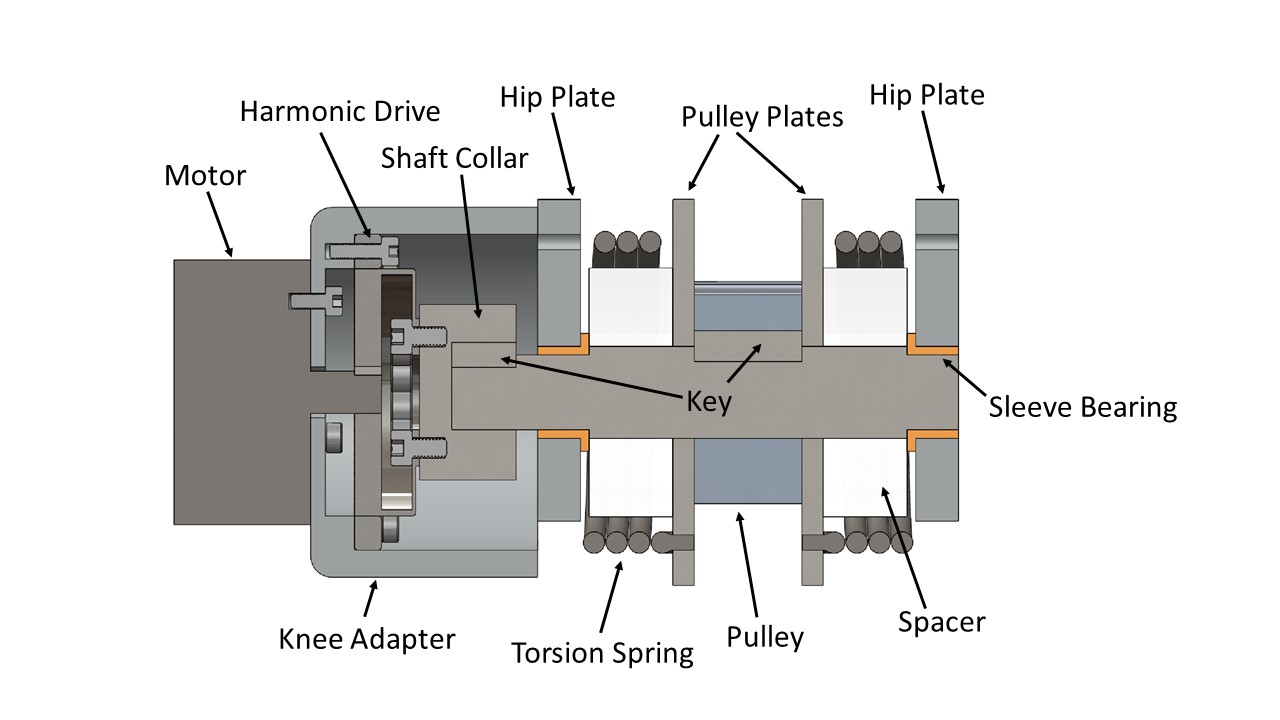
\includegraphics[width=\textwidth]{2_ProposedDesign/img/SectionHipKneeShaftA.jpg}
    \caption{Section view of knee control shaft and its adaptor}
    \label{fig:shaft_kneehip} 
\end{figure}



\begin{comment}
\subsubsection{Assembly of the O-Crab}

The O-Crab was designed to take into account the assembly process of the various parts. First, alignment of the various shafts is ensured by assembling the two hip plates together with locating pins, machining the shaft holes and then taking the plates apart again. The same is done with the hip bracket, base plate and adaptor assembly. 

To assemble, the sleeve bearings can first be press fit into the hip plates and hip brackets. The foot is assembled onto the tibia tube and then the tube is press fit into the tibia holder. Then, the belt must be positioned on the exterior pulley and the pulley slipped between the tibia holder arms. This assembly can be slipped on the exterior knee shaft, followed by the spacers. The belt is then positioned on the interior pulley and the knee control shaft is assembled. The hip control shaft must only be partly assembled for now, by positioning only the middle spacer. 

The next step is to position all the shafts onto the hip plates, and to bolt the two hip plates together at the alignment pins. The tensioner is added on the belt to remove any slack. The other spacers and the springs can then be added onto the hip control shaft. The hip brackets are then inserted on either side and bolted onto the base plate.

The motors are then attached each to their respective adaptor. The Harmonic Drives are attached to the shaft collars, and then to their adaptor. These assemblies are then inserted onto the shafts by their shaft collars. The knee adaptor is bolted onto the hip plates and the hip adaptor is bolted onto the base plate. The full leg assembly can then be assembled onto the chassis by slipping the tibia through the leg hole and fastening the base plate to the chassis. The bellow is installed afterwards with hose clamps. Once all legs are installed, the electronics can be added.

\end{comment}
